\chapter{GIỚI THIỆU}
\label{Chapter1}

\section{Đặt vấn đề}

% Ngữ cảnh, vấn đề cần giải quyết là gì?
Các quản trị viên \acrfull{vnpt} yêu cầu xây dựng hệ thống \acrfull{iot} giám sát các \acrfull{bts}. Hệ thống \acrshort{iot} phải cung cấp bo mạch giám sát thông số của các trạm \acrshort{bts}, giao diện người dùng dựa trên cơ sở dữ liệu của \acrfull{vps}, và có sử dụng mật mã hóa.

Trong quá trình phát triển, mô hình hệ thống phần cứng và các cơ chế giao tiếp và đồng bộ trên phần cứng phải được thiết kế. Tại \acrshort{vps}, mô hình hệ thống back-end và nền tảng giao diện người dùng phải được xác định. Bên cạnh đó, hệ thống phải đưa ra loại mật mã hóa được sử dụng. Trong quá trình hoạt động, bo mạch in phải được thiết kế để phù hợp với việc giám thông số của trạm \acrshort{bts} và có thể triển khai cơ chế đồng bộ với back-end system. Tại \acrshort{vps}, kỹ thuật triển khai hệ thống back-end và nền tảng giao diện phải được đưa ra. Cuối cùng, hệ thống \acrshort{iot} phải đưa ra cách thức triển khai kỹ thuật mật mã hóa.

% Vì sao vấn đề/bài toán quan trọng và thú vị?
    % Quản trị viên VNPT muốn giám sát BTS online.
Khi yêu cầu xây dựng hệ thống \acrshort{iot}, các quản trị viên muốn giám sát trạm \acrshort{bts} online thay vì giám sát trực tiếp. Chính vì vậy, hệ thống \acrshort{iot} sẽ phục vụ cho việc giảm thiểu việc giám sát trạm \acrshort{bts} offline và chi phí di chuyển tới trạm. 
    % Hệ thống IoT giải quyết vấn đề của BTS và các vấn đề khác.
Không chỉ phục vụ cho việc giám sát trạm \acrshort{bts}, hệ thống \acrshort{iot} sẽ được xây dựng với cấu trúc linh hoạt để phục vụ nhiều loại hệ thống giám sát và điều khiển online.

% Bài toán có gì khó? Vì sao cần phải giải quyết?
    % Cơ chế giao tiếp và đồng bộ đáng tin cậy và tự phục hồi
    % Giao diện người dùng phải linh hoạt để dễ dàng thay đổi các thành phần hiển thị.
    % Hệ thống back-end phải đồng bộ các dữ liệu của cơ sở dữ liệu với giao diện và bo mạch.
    % Giúp cài đặt cơ chế đồng bộ và giao tiếp trên toàn hệ thống. Triển khai mật mã nhẹ một cách hợp lý
Trong việc giao tiếp, hệ thống phải có cơ chế giao tiếp và đồng bộ đáng tin cậy và có khả năng tự phục hồi. Hơn nữa, giao diện người dùng phải linh hoạt để dễ dàng thay đổi các thành phần hiển thị của người dùng. Sau cùng, hệ thống back-end phải có cơ chế đồng bộ dữ liệu với giao diện và bo mạch một cách đáng tin cậy. Khi giải quyết được các vấn đề trên, cơ chế giao tiếp và đồng bộ có thể triển khai trên toàn hệ thống và có thể triển khai mật mã hóa hợp lý.

\section{Mục tiêu}

% Thiết kế bo mạch sử dụng vi điều khiển và phù hợp với việc giám sát BTS.
% Thiết kế cơ chế đồng bộ đáng tin cậy và có khả năng tự phục hồi. Cấu trúc frame có các thành phần nhận diện và phát hiển lỗi.
% Giao diện web linh hoạt có thể tùy chỉnh các thành phần hiển thị.
% Mật mã hóa được triển khai hợp lý trên cơ sở giao tiếp.
% Thiết kế hệ thống back-end có cơ sở dữ liệu, API server, và web-server.
Bo mạch hướng tới thiết kế sử dụng \acrfull{mcu} cấu tạo nên các thiết bị và gateway phù hợp với viêc giám sát \acrshort{bts}. Về việc giao tiếp, cơ chế đồng bộ được xây dựng đáng tin cậy và có khả năng tự phục hồi. Hơn nữa, cấu trúc frame giao tiếp được tạo nên có các thành phần nhận diện frame và phát hiện lỗi. Về bảo mật, mật mã hóa được triển khai hợp lý trên cơ sở giao tiếp của hệ thống. Về giao diện, hệ thống cung cấp giao diện web linh hoạt có thể tùy chỉnh các thành phần hiển thị. Về hệ thống back-end, back-end cung cấp cơ sở dữ liệu, \acrshort{api} server, broker server, và web-server.

\section{Giải pháp}

% Những giải pháp (nghiên cứu, ứng dụng) đã giải quyết bài toán này?
    % Các IoT Cloud như Blynk, ThingsBoard được sử dụng để thu nhận và trực quan hóa dữ liệu từ bo mạch.
    % Sử dụng vi điều khiển ESP Station ở chế độ Web-Server.
Các \acrshort{iot} cloud như Blynk và ThingsBoard được sử dụng để thu nhận, quản lý và trực quan hóa dữ liệu từ bo mạch. Ngoài ra, ESP32 web-server ở chế độ station là giải pháp giám sát và điều khiển thiết bị trong phạm vi nhỏ (xung quanh một Access Point).

% Những giải pháp này có hạn chế, thiếu sót gì?
    % Blynk không thể triển khai mật mã hóa tùy chỉnh vì không có open-source back-end.
    % ThingsBoard có open-source nhưng dung lượng back-end lớn hơn khả năng tải của máy chủ ảo của các quản trị viên.
    % ESP32 không đủ khả năng host back-end phục vụ nhiều thiết bị.
Việc sử dụng Blynk cloud không thể triển khai kỹ thuật mật mã hóa tùy chỉnh do nền tảng không có open-source back-end. Đối với ThingsBoard platform, nền tảng ThingsBoard cung cấp open-source cho hệ thống back-end nhưng kích thước back-end này lơn hơn khả năng tải của \acrshort{vps} của các quản trị viên \acrshort{vnpt}. Trên ESP32, \acrshort{mcu} ESP32 không đủ khả năng host một back-end phục vụ nhiều thiết bị ở các \acrshort{bts}.

% Giải pháp của bạn là gì? Kết quả thế nào?
    % Mô hình: cấu trúc 4 lớp
Mô hình của hệ thống được thiết kế theo mô hình IoT 4 lớp (minh họa như hình \ref{fig:IoT-4-Layer-Archi}). Theo mô hình này, hệ thống IoT bao gồm 4 lớp chính: Perception Layer, Network Layer, Processing Layer, và Application Layer. Mô hình IoT được triển khai ở các Access Point và \acrshort{vps}, và sử dụng các kết nối có dây và không dây (mô tả hình \ref{fig:IoT-Connections-Model}).

    % Phần cứng
    % mô hình back-end
    % giao diện
    % giao tiếp và đồng bộ
    % mã hóa
Cụ thể, tại perception layer, phần cứng của hệ thống là bo mạch của \acrfull{ptn} DESLab và sử dụng \acrshort{mcu} ESP32 và STM32 và các cảm biến đo nhiệt độ, dòng điện, điện thế, và contactor. Trong đó, STM32 là thiết bị giao tiếp vạn vật và ESP32 là \acrshort{iot} gateway.
% 
Tại \acrshort{vps} (network layer), hệ thống back-end là tập hợp của \acrfull{mqtt} Broker, MongoDB database, và EggJS server, và back-end được triển khai bằng kỹ thuật Docker Containerizing. Tại application layer, Nginx web-server được triển khai để cung cấp giao diện web trực quan hóa dữ liệu thiết bị cho người dùng.
%
Cụ thể, giao diện người dùng là giao diện web được xây dựng trên cơ sở của nền tảng Ant Design Pro và có các thành phần giao diện có thể tùy chỉnh và kéo thả.
%
Về giao tiếp và đồng bộ trong processing layer, hệ thống sử dụng cơ chế giao tiếp có các thành phần nhận diện frame và phát hiện lỗi. Từ đó, cơ chế giao tiếp có độ tin cậy và tự phục hồi, và triển khai giữa EggJS server, bo mạch, và giao diện web.
%
Tiếp theo, cơ chế đồng bộ được triển khai dựa trên sự kiện ``change stream'' của MongoDB và giữa EggJS server, bo mạch, và giao diện web.
%
Cuối cùng, cũng trong processing layer, mật mã hóa nhẹ ChaCha20-Poly1305 được sử dụng trên giao tiếp giữa \acrshort{iot} gateway ESP32 và EggJS server.

\begin{figure}[htp]
\centering
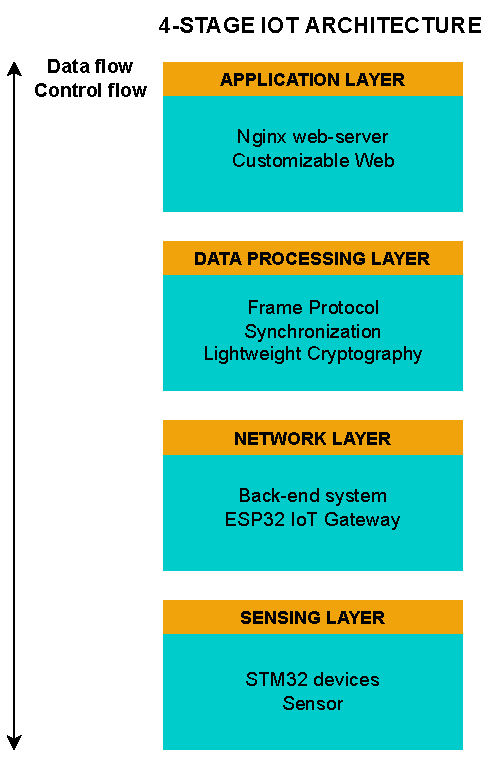
\includegraphics[width=8 cm]{images/Thesis-Page-2-IoT-Archi.pdf}
\caption{Mô hình 4 lớp của hệ thống IoT. Nguồn tham khảo InterviewBit~\cite{IoT-4-Layer-Archi}}
\label{fig:IoT-4-Layer-Archi}
\end{figure}

\begin{figure}[htp]
\centering
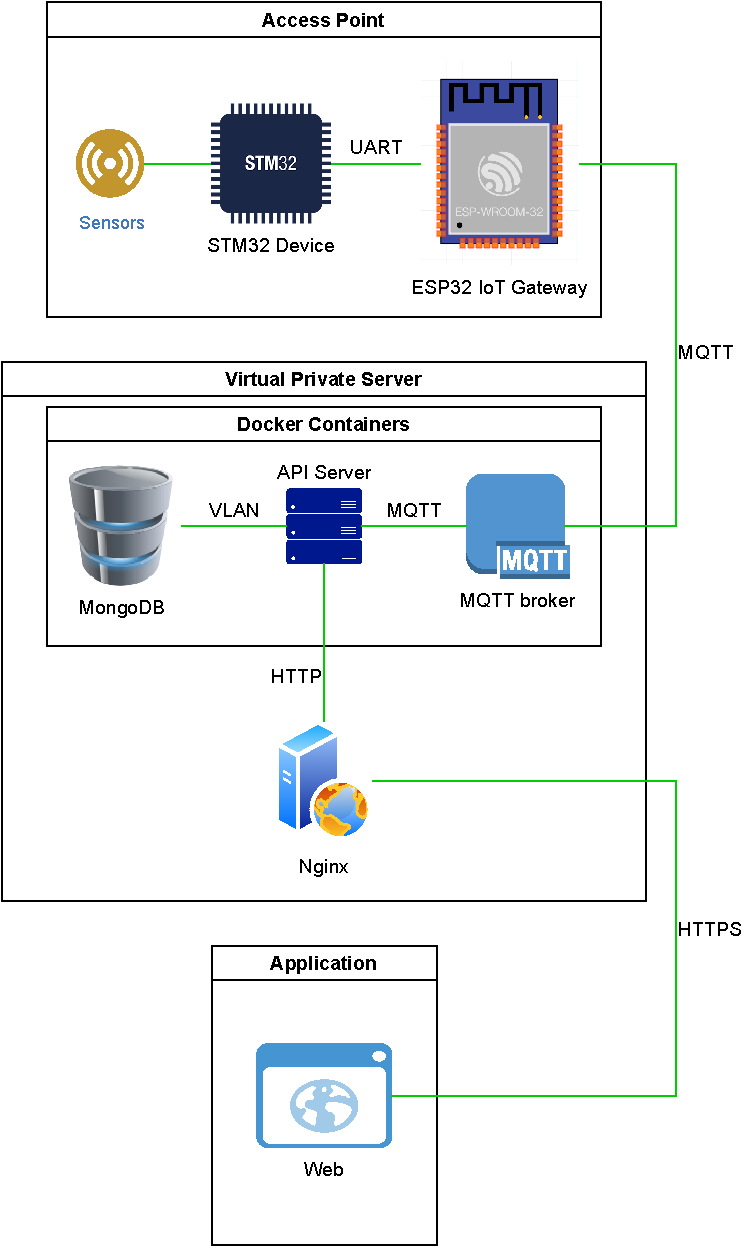
\includegraphics[width=0.75\linewidth]{images/Thesis-Page-3-IoT-Connections-Model.pdf}
\caption{Mô hình kết nối và giao thức của hệ thống IoT.}
\label{fig:IoT-Connections-Model}
\end{figure}

\section{Đóng góp}

% Đóng góp của nghiên cứu/ứng dụng của bạn?
    % Triển khai kỹ thuật giao tiếp và đồng bộ ở thiết bị STM32, gateway ESP32, và API server.
    % Triển khai kỹ thuật mật mã hóa nhẹ ChaCha20-Poly1305 trên gateway ESP32 và API server.
    % Phát triển hệ thống back-end và giao diện web.
    % Sử dụng kỹ thuật docker containerizing triển khai hệ thống back-end và nginx web-server cung cấp giao diện web
Kết quả của khóa luận này là những đóng góp trong kỹ thuật giao tiếp-đồng bộ, phát triển và triển khai hệ thống back-end và giao diện web. Trong giao tiếp-đồng bộ, kỹ thuật giao tiếp-đồng bộ đã được triển khai trên thiết bị STM32, gateway ESP32, và \acrshort{api} server. Trong mật mã hóa, kỹ thuật mật mã hóa nhẹ ChaCha20-Poly1305 đã áp dụng trên giao tiếp giữa gateway ESP32 và \acrshort{api} server. Trên hệ thống back-end, \acrshort{mqtt} broker và \acrshort{api} server được phát triển trên nền tảng NodeJS. Hơn nữa, kỹ thuật Docker containerizing được sử dụng để triển khai các thành phần của hệ thống back-end. Cuối cùng, về giao diện, giao diện được phát triển trên nền tảng Ant Design Pro và ngôn ngữ TypeScript, và được triển khai bằng máy chủ web Nginx.

\section{Bố cục}

Báo cáo khóa luận được chia thành 5 chương. Đó là:
\begin{itemize}
    \item Chương \ref{Chapter1}: GIỚI THIỆU.
    \item Chương \ref{Chapter2}: CÁC HỆ THỐNG VÀ CÔNG NGHỆ LIÊN QUAN.
    \item Chương \ref{Chapter3}: \textsc{\tenKL}.
    \item Chương \ref{Chapter4}: KẾT QUẢ.
    \item Chương \ref{Chapter5}: KẾT LUẬN.
\end{itemize}

Đầu tiên, chương \ref{Chapter1} đưa ra các nội dung tổng quát của khóa luận. Các nội dung bao gồm việc đặt vấn đề, mục tiêu đề ra, giải pháp đề xuất, đóng góp, và bố cục của khóa luận.

Tiếp theo, chương \ref{Chapter2} đưa ra các đánh giá và khảo sát các hệ thống \acrshort{iot} trong việc giải quyết vấn đề của khóa luận. Hơn nữa, chương này còn đưa ra mô hình hệ thống \acrshort{iot} được đề xuất và các lý thuyết xây dựng hệ thống \acrshort{iot} được đưa ra.

Trong việc triển khai hệ thống, chương \ref{Chapter3} trình bày các phương pháp và giải phát đề xuất đề xây dựng hệ thống \acrshort{iot}. Các nội dung này trình bày các phương pháp và giải pháp trên việc xây dựng mô hình, bo mạch, giao diện web, và hệ thống back-end.

Về các kết quả, chương \ref{Chapter4} đưa ra các kết quả đã đạt được trên phần cứng, \acrshort{vps}, và giao diện web.

Cuối cùng, chương \ref{Chapter5} đưa ra các mô tả ngắn gọn về mục tiêu, phương pháp, kết quả đạt được, ý nghĩa của kết quả cũng như những hạn chế, giới hạn của đề tài và hướng phát triển.

%Tóm tắt luận văn được trình bày nhiều nhất trong 24 trang in trên hai mặt giấy, cỡ chữ Times New Roman 11 của hệ soạn thảo Winword hoặc phần mềm soạn thảo Latex đối với các chuyên ngành thuộc ngành Toán.

%Mật độ chữ bình thường, không được nén hoặc kéo dãn khoảng cách giữa các chữ.
%Chế độ dãn dòng là Exactly 17pt.
%Lề trên, lề dưới, lề trái, lề phải đều là 1.5 cm.
%Các bảng biểu trình bày theo chiều ngang khổ giấy thì đầu bảng là lề trái của trang.
%Tóm tắt luận án phải phản ảnh trung thực kết cấu, bố cục và nội dung của luận án, phải ghi đầy đủ toàn văn kết luận của luận án.
%Mẫu trình bày trang bìa của tóm tắt luận văn (phụ lục 1).